%\comment{A conclusion section is not required. Although a conclusion may review the main points of the paper, do not replicate the abstract as the conclusion. A conclusion might elaborate on the importance of the work or suggest applications and extensions.}


%The main contribution of this paper is a technique to learn the inverse dynamics model of robots under the effect of multiple and simultaneous contacts exerted on the whole robot structure. 
%In whole-body robot control, estimating contact forces accurately is crucial
%may not only be understood as nuisance that need to be avoided. Making contacts may rather be seen as a desirable feature 
%for balance and stabilization, and to increase the number of potential actions that the robot is able to execute, e.g., reach for distant objects.
%, to stabilize or even . 
Whole-body control strategies that exploit contacts need accurate models of the system dynamics.
%to be stable and precise. 
This is crucial for balance and stabilization, and to increase the number of potential actions that the robot is able to execute, e.g., creating a contact to reach for distant objects.
%
We introduced a data-driven mixture-of-experts approach based on Gaussian processes  for learning inverse dynamics models with contacts. 
% A  was proposed to deal with multiple contacts. %model these non-linear effects. 
We evaluated our model on the \robot{} humanoid robot using tactile sensors and force/torque sensors as model inputs.  
We showed that the model accurately predicts contact forces and outperforms a state-of-the-art analytical approach used to estimate the joint torques in \robot{}. 
The estimation from the learned model does not rely on dynamic parameters, but it is completely data-driven and based on tactile sensors and force/torque sensors. %to determine the amount of external forces.
As a result, our approach does not require a spatially calibrated model of the skin~\cite{DelPrete2011,DelPrete2012}.
% Neither spatially calibrated models of the skin~\cite{DelPrete2011,DelPrete2012} nor preceise knowledge about the contact location were required --- in contrast to the analytical modeling strategy. 
This is a promising feature for robust control strategies that explicitly takes contacts into account. 
%In future, we will incorporate our inverse dynamics models in active control tasks involving multiple contacts in whole-body structure, such as balancing with multiple supports in rigid and compliant environments.

% In future work, we will incorporate our inverse dynamics models in active control tasks using rewards as training signals to overcome the need of labels or ground truth data.

%, which involve multiple simultaneous contacts.
%and as such we could utilize the mixing property of the experts.

% Our solution enables a fast and accurate prediction of the joint torques in situations when the robot is in contact (or not) with an object, detected by a tactile skin.
% The estimation from the learned model does not rely on dynamic parameters, but it is completely data-driven by using tactile sensors and force/torque sensors to determine the amount of external forces.
% As a result, our approach does not requires a spatially calibrated model of the skin~\cite{DelPrete2011,DelPrete2012}.
% With the increasing availability of larger arrays of skin sensors, this kind of data-driven approach greatly reduces the design/engineering complexity.
% %
% %It only introduces an additional sensor measurement $\skinInput$, which provides the information about the contact location and a measure of the applied force on the taxels. 
% Moreover, tactile sensors are cheaper and lighter than joint torque sensors. 
% With our approach, it is possible to apply torque control to robotic manipulators even with contacts at locations other than the end-effector, which makes it possible to control the robot while physically interacting with an evolving environment or humans.

% \todo[inline]{kill this paragraph?\\
% Another advantage of our data-driven approach is that model predictive control needs rapid computation, since it has to compute the entire robot dynamics over a receding time horizon at each control step (as in \cite{naveau2014metapod}, within 1--2~$\mu$s).
% The use of a learned model such as GP potentially allows to reduce the computational time at prediction time and hence to be beneficially used in fast real time applications.}

	%
	\begin{figure}[t]
			\centering
			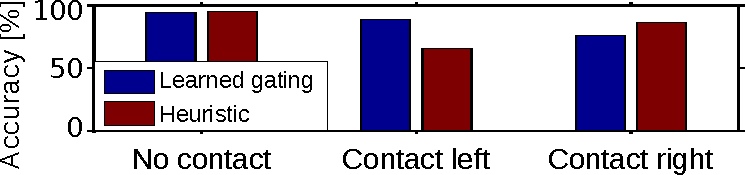
\includegraphics[width=.94\hsize]{fig/exp5_accuracy_red}
		\caption{\textbf{\nameref{sec:results:exp5}:} Classification accuracy for the heuristic and learned SVM gating networks.
		}
		\label{fig:exp5:accuracy}
        \figspace
	\end{figure}
	%